\documentclass[11pt, a4paper]{article}
\usepackage[T2A]{fontenc}
\usepackage[utf8]{inputenc}
\usepackage[english]{babel}

%% Sets page size and margins
\usepackage[a4paper,top=3cm,bottom=3cm,left=3cm,right=3cm,marginparwidth=1.75cm]{geometry}

%% Useful packages
\usepackage{amsmath, amssymb, amsthm,calc,mathabx}
\usepackage{systeme}
\usepackage{graphicx}
\usepackage[colorinlistoftodos]{todonotes}
\usepackage[colorlinks=true, allcolors=black]{hyperref}
\usepackage{wrapfig,lipsum,booktabs}
\usepackage{enumitem}
\usepackage{float}
\usepackage{fmtcount}
\usepackage{multicol}
\usepackage{breqn}
\usepackage{setspace}
\usepackage{hyperref}
\usepackage{mathtools}
\usepackage {tikz}
	\usetikzlibrary {positioning}
	\usetikzlibrary{shapes.geometric}
\graphicspath{
	{Graphics/}
	{Graphics/BackupFunction/}
}
\newtheorem{theorem}{Theorem}

\newtheorem{lemma}{Lemma}
\newtheorem{prop}{Property}
\newtheorem*{remark}{Remark}

\theoremstyle{definition}
\newtheorem{definition}{Definition}

\setlength{\columnsep}{1cm}
\setlength{\parindent}{1em}

\newcommand\blfootnote[1]{%
	\begingroup
	\renewcommand\thefootnote{}\footnote{#1}%
	\addtocounter{footnote}{-1}%
	\endgroup
}

\begin{document}
\begin{titlepage}
	\newcommand{\HRule}{\rule{\linewidth}{0.5mm}}
	\centering
	\textsc{\LARGE Innofair 2019}\\[1cm]
	\HRule\\[1 cm]
	{\huge\bfseries On Ransomware and Resilient Backup Strategies}\\[0.5 cm] 
	\HRule\\
			\vfill
			\Large
			\textit{Author:}
			\textsc{Nikola Staykov}\\
            \vspace{2cm}
			\Large
			\textit{Supervisor:}
            \textsc{Yavor Papazov}\\
            
\includegraphics[width=0.5\textwidth]{Innofair_logo}\\
    \vfill	
	{\large\today}   
	\vfill
\end{titlepage}

\tableofcontents
\newpage
\begin{abstract}
		Ransomware is a type of computer virus, which encrypts the files on a given system and asks for a ransom in order for them to be decrypted. Ransomware authors  can make small surveys before launching the main campaign, in order to estimate the distribution of the prices people are willing to pay. The first part of the paper explores a model, which aims to find the most suitable parameters for such a survey. The main and most efficient defence against ransomware is simply to backup your data. Backups however, can create significant costs for big companies and should therefore be well scheduled, which is taken into account in the second part of the paper. A model for backing up data is considered, consisting of full and incremental backups, and the expected recovery price is calculated. The backup recovery process has been recreated and analyzed using a python visualization and a Monte Carlo simulation.
\end{abstract}

\section{Introduction}
	This project is structured in two main parts, considering respectively models for ransom optimization and backup optimization. By thoroughly examining both viewpoints in a situation, a full picture of the strategies of both the attackers and the victims has been created. Considering ways both sides can optimize their profits and expenses gives us insight on how to build a solid backup strategy.
\section{Preliminaries}
	In this section are stated all the needed definitions and concepts one needs to fully understand the paper.
		\begin{definition}
			\label{def:normdist}
			\emph{Normal Distribution}, denoted by $N(\mu, \sigma)$, is a type of continuous distribution, such that $\mu$, $\sigma$ and $\sigma^{2}$ denote the mean, the standard deviation and the variance, respectively.
		\end{definition}
	
		The graph of this function forms a curve, often called informally bell curve. It has maximum $(x,f(x))$ at $\left(\mu, \dfrac{1}{\sigma\sqrt{2\pi}}\right)$:
		\begin{center}
			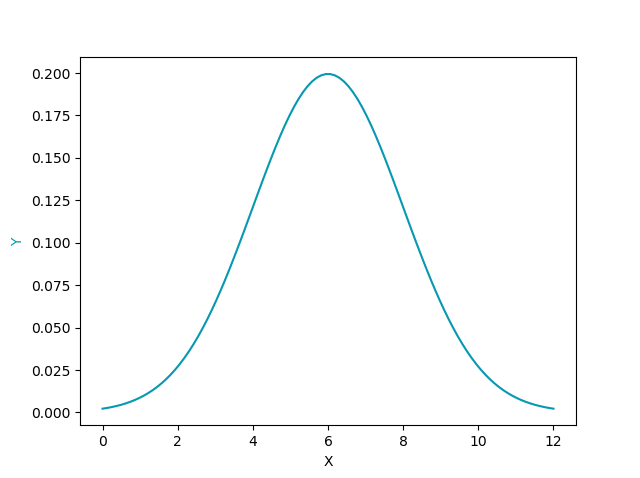
\includegraphics[width=0.6\textwidth]{Normal_clean}
		\end{center}
		
		\begin{definition}
			\label{def:def2}
			Consider a normal distribution $N(\mu, \sigma)$. The \emph{standard value}, or the \emph{Z-score}, of a given $x$ evaluates how many standard deviations away from the mean the given value is. It is computed by $\dfrac{x-\mu}{\sigma}$.
		\end{definition}
	
		\begin{definition}
			\label{def:prob_dist}
			For a given distribution the \emph{probability distribution function} $F(x)$ calculates the probability that a random variable, following the distribution, is less or equal to $x$
			$$F_{X}(x)=\mathbb{P}(x\leq X).$$
		\end{definition}
	
		\begin{definition}
			\label{def:prob_dens}
			The \emph{Probability density function} of a continuous random variable $x$, a probability density function describes the probability a random variable $x$ to appear in any interval. Formally it is defined by
			\begin{align*}
				&\mathbb{P}(x < X \leq x+\Delta)=F_X(x+\Delta)-F_X(x)\\
				&f_X(x)=\lim_{\Delta \rightarrow 0} \frac{F_X(x+\Delta)-F_X(x)}{\Delta}.		
			\end{align*}
		\end{definition}
	
		\begin{definition}
			\label{def:err}
			\emph{The error function} is encountered in integrating the normal distribution, it takes z-score as a parameter and calculates the integral between a fixed point and the mean of the distribution
			$$\operatorname{erf}(z)=\dfrac{2}{\sqrt{\pi}}\int_{0}^{z}e^{-t^{2}}dt.$$
		\end{definition}
	
		\begin{definition}
			\label{def:Bernoulli_trial}
			\emph{A Bernoulli trial} is a random experiment with two outcomes and fixed probability of failure and therefore success:
			\begin{center}
			$P(\text{success})=p$\\
			$P(\text{failure})=1-p.$
			\end{center}
		\end{definition}
	
		\begin{definition}
			\label{def:Binomial_distribution}
			\emph{A binomial distribution} is the statistical distribution of outcomes(success/failure) when conducting a number of independent Bernoulli trials.
			For $n$ trials and success probability $p$ the probability that exactly $k$ of them are successful is:
			$$
			P(\text{success} = k) = \frac{\binom{n}{k}p^{k}(1-p)^{n-k}}{2^k}
			$$
		\end{definition}
\newpage
	\section{Ransom optimization}
		\subsection{Introduction}
			Ransomware first appeared in 1989 in the form of the AIDS Troyan, aka PC Cyborg.  The AIDS Trojan was pretty easy to overcome as it used simple symmetric cryptography and tools were soon available to decrypt the files, but this case set the ground for a lot of the modern threats. With the coming of the Internet age, ransomware returned with new power, namely with the Archiveus Trojan and GPcode from 2006. Another turning point in the history of ransomware was the invention of bitcoin, and crypto-currencies as a whole, for several reasons, a few of them being anonymity, the transactions are fully automatable and the transactions are irrefutable\cite{huang2018tracking}.\par
			In the recent years there have been some attempts to model the ransomware market. In \cite{caulfielddynamic}, the authors have created a theoretical model, taking into consideration the number of users, who have backups, as well as other factors such as information spread and reliability of the ransomware.\par                 
			In \cite{cartwright2018pay} a different approach has been explored, considering the possibility for bargaining and respectively a game between the victim and the criminals. This paper focuses on game theory and combinatorics.\par
			There has also been considerable amount of effort dedicated to tracking the ransomware payments in the blockchain, as all of them are public. As a result, there is a public data record of such payments, provided by \cite{paquet2019ransomware} and in \cite{thomas2015framing} many one can observe many data-based conclusions not only concerning ransomware, but also the whole black market.\par
			In this paper, the model is based on the one described in \cite{caulfielddynamic}, but focuses on optimizing different parameters, unexplored in the aforementioned research.
		\subsection{Approach}
			This model describes the spreading of a ransomware virus. It calculates the optimal ransom for a ransomware attack, distributed exclusively via botnets, without the key component of spreading to every computer in the network. This variant of the attack is relatively cheap to initiate, but has low efficiency.	We treat the act of decrypting the data of a given computer as a service and the ransom as the service price, respectively. \par
			Consider the distribution of the willingness to pay (WTP) of a given target group. This is the maximum price someone would pay for their data. By putting ourselves in the place of the ransomware authors, we try to find what the distribution is by examining samples of people and how they respond to a given price. This tests, however, cost us valuable time since the awareness of people rises constantly. We strive to determine how many and how big tests should we conduct in order to model the distribution with reasonable error and in the same time not lose too much time?\par
			For a given size of the sample group, we calculate the error of a set of sample `customers' from the mathematically described function of the demand curve, derived from the distribution of WTP. Starting off low, we gradually expand the sample group size, estimating the expected error, via the Least Squares Approach, at each step.
	\newpage
		\subsection{Model}
			Here the inner workings of the model are stated in detail, showing how the results and conclusions were reached. The section is divided into two parts, corresponding to the parameters the model explores.
			\subsubsection{Sample size and error}
			This section describes the mathematical model, used to optimize the error and draw conclusions about the sample size.\par
			We assume people's data value follows a normal distribution and link it to a random variable $p\sim N(500, 150)$. The probability density function (PDF) of a normal distribution $N(\mu, \sigma)$ is $$\frac{1}{\sigma\sqrt{2\pi}}e^{-\frac{(x-\mu)^{2}}{2\sigma^{2}}}.$$\par\noindent
			In order to calculate the demand function $f(k)$ from the PDF for a given price $k$, we need to calculate
			$$\int_{k}^{\infty}f(x)\operatorname{d} x.$$
			\begin{figure}[H]
				\begin{minipage}{0.48\textwidth}
					\centering
					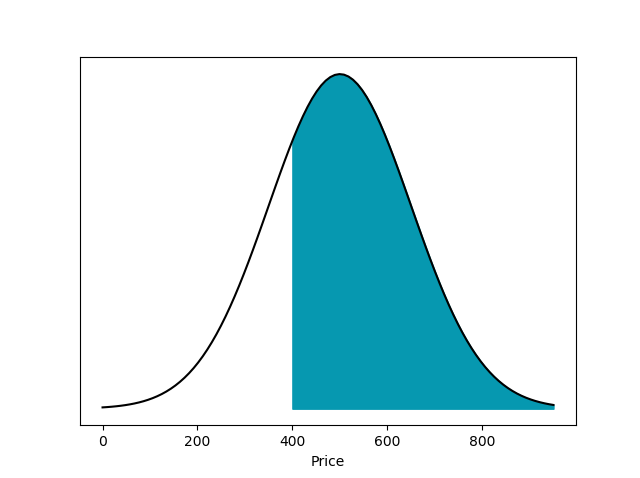
\includegraphics[width=\linewidth]{ND_integral}
					\caption{PDF}\label{Fig:Data1}
				\end{minipage}$\longrightarrow$
				\begin{minipage}{0.48\textwidth}
					\centering
					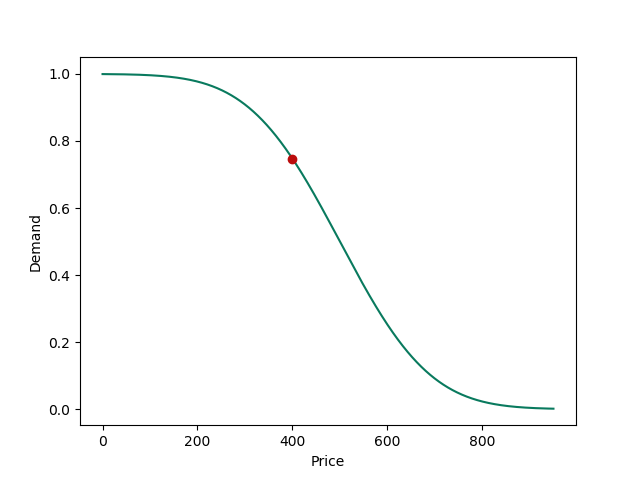
\includegraphics[width=\linewidth]{Sample_point}
					\caption{Price vs Demand}\label{Fig:Data2}
				\end{minipage}
			\end{figure}\par\noindent
			We note that the integral must be calculated up to infinity, but after $k$ reaches $\mu+3\sigma$, the resulting integral is negligibly small. Doing this for the whole probability distribution function gives us the demand curve with respect to what percent of the people would pay. Let us denote the demand curve function with $F(x)$:
			$$
			F(x)=
			\begin{cases}
				\dfrac{1}{2}\left (1-\operatorname{erf}\left (\dfrac{z}{\sqrt{2}}\right )\right ) \text{if } x>\mu,\\
				\\
				\dfrac{1}{2}\left (1+\operatorname{erf}\left (\dfrac{z}{\sqrt{2}}\right )\right ) \text{if } x<\mu.
			\end{cases}
			$$\par
			We aim to optimize the number of people each sample group consists of. Knowing the actual mathematical function we aim to describe gives us the possibility to evaluate the errors from the experimental data with maximum accuracy.
			\begin{figure}[H]
				\begin{minipage}{0.48\textwidth}
					\centering
					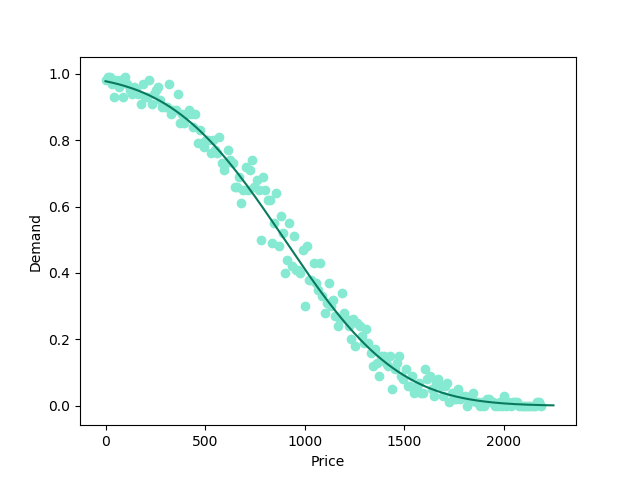
\includegraphics[width=\linewidth]{Exp_and_math_100}
					\caption{Sample size 100}\label{Fig:Data3}
				\end{minipage}\hfill
				\begin{minipage}{0.48\textwidth}
					\centering
					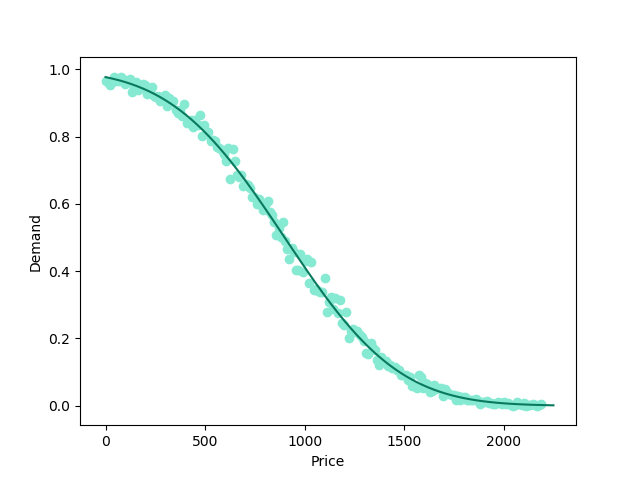
\includegraphics[width=\linewidth]{Exp_and_math_400}
					\caption{Sample size 400}\label{Fig:Data4}
				\end{minipage}
			\end{figure}\par\noindent
			By gathering information on the sample size and the corresponding errors, we plot the changes in the error.
			\begin{figure}[H]
			\begin{minipage}{1.0\textwidth}
				\centering
				\includegraphics[width=0.7\textwidth]{"Error vs sample size 4"}
				\caption{Sample size vs Error}\label{Fig:Data5}
			\end{minipage}
			\end{figure}	
			%\subsubsection{Backup function}
			%	In this section a function, describing the use of backups, is described. The effect on revenue is calculated.\par
			%	First let us define the backup iterator $b$: 
			%$$
			%b=
			%\begin{cases}
			%	1 \text{ if the victim has backup},\\
			%	0 \text{ if the victim does not have backup}
			%\end{cases}
			%$$
			%Now let us define the willingness to pay (WTP) function:
			%$$
			%P(x)=
			%\begin{cases}
			%d_{x} \text{ if } b_{i}=0,\\
			%c \text{ if } b_{i}=1
			%\end{cases}
			%$$
			%	Here the cost of backup is denoted with $c$ and the value of the victim's data - with $d_{x}$.\par
			%	As earlier, we can calculate the expected probability of people paying a ransom of price $x$
			%	We assume that the probability that a single victim has backup follows is $p$ and explore how changing this value affects the expected profit. With the gathered data, we create a plot to show the correlation between the two variables
			%\begin{center}
			%	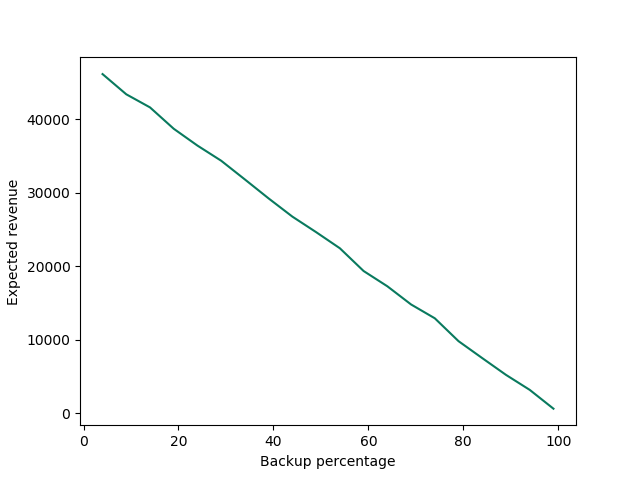
\includegraphics[width=0.55\textwidth]{Revenue_vs_backup}
			%\end{center}
		\subsection{Results}
		We have explored how the sample size affects the expected error between the statistical and experimental data and have explored how backups affect expected revenue. The model mainly focuses on optimizing the ransom prize, but the author truly believes that in order for us to be able to take countermeasures against ransomware attacks, we need to understand their every move and essential for the purpose. We can use the gathered data to create a resilient backup strategy.
\section{Backup optimization}
	\subsection{Introduction}
		When it comes to protection from ransomware, the most efficient method is building backups. This, however, has to be done regularly, as the effects after a potential attack will otherwise be insignificant. That is why it is important for backup protocols to be carefully build, considering both the risks of being attacked and the resources needed for the job. Furthermore, optimizing the backups can simultaneously increase the security level and save money.\par
		In this section, a model for backing up data is considered in order to calculate the expected price. Such models, considering two options for backups: full and incremental, have been constructed and researched in the past\cite{nakamura2003optimal}\cite{qian2010optimal}. We consider a cycle of backups, which repeats over between any two full backups and study how the intervals affect the expected price and how fast the effect of initial data, accumulated before the initial full backup, vanishes over time.
	\subsection{Theoretical setting}
		The idea behind the described model is to calculate and optimize the expected price of the recovery in case of an attack.\par
		We will consider a backup as a structure, containing the following properties:
		$$
		B
		\begin{cases}
			d \text{: the date on which the backup was made, as a day difference from a starting point}\\
			p \text{: the probability that the recovery is unsuccessful for any reason}\\
			r \text{: the price of trying to recover the data from the given backup}
		\end{cases}
		$$
		
		Two types of backup will be considered:
		\begin{enumerate}
			\item Full backup: a backup of the whole database
			\item Incremental backup: only saves the changes from the last backup
		\end{enumerate}
		The backups from a certain type share common probability of failure and price for a recovery try.\par
		In order for an incremental backup to be successful, all the incremental backups which precede it up to a full backup need to be successful as well as the full backup itself.\par
		In this case data value should clearly be taken into account from a subjective point of view. Even though on the market some data may not be worth a lot, if it is essential for the functioning of a given company, it is clear that it will be willing to pay a lot to regain access to it immediately. Therefore, in the described model data value is considered as an ever-increasing amount, for the purposes of the research the "work rate", namely the data value generated in a day, of the company is taken as a constant. We will denote it with $w$.\par
		The cost of a backup recovery will be considered as a sum of two factors:
		\begin{itemize}
			\item The cost of redoing the lost work, denoted with $W$
			\item The cost of the recovery process itself, denoted with $R$
		\end{itemize}.
		We define $W = \Delta t.w$, where with $\Delta t$ we denote the difference in days between the successful backup and the disaster date and $R = \sum_{i=1}^{n} r_i$, where the number of attempted backups is $n$ and 
		$$
		S=\Delta t.w + R,
		$$
		Let the difference in days from the first backup to the disaster date be $T$. In case none of the backups are successful, we consider a variable $W_T$, corresponding to the price of redoing the whole work the company has done from the beginning. It is clear that $W_T>T.w$\par
		\subsection{Full backups only}
		When we only consider a set of full backups, the model is simply a Bernoulli distribution with finite trials, namely the number of full backups. We stop when we find a successful backup, starting from the latest and going to the last. Let us define the properties of a full backup($B_F$):
		$$
		B_F
		\begin{cases}
			p_F: \text{the probability of failure}\\
			r_F: \text{the recovery trial cost}\\
			t_F: \text{the days between two consecutive full backups}\\
		\end{cases}
		$$
		Let $k$ be the number of full backups made before the disaster date. Then:
		$$
			k = \left \lfloor{\frac{T}{t_F}}\right \rfloor + 1
		$$
		We can now define the expected backup cost:
		\begin{equation}
		\label{eq:1}
			E(T) = p_F^{k}\left(W_T + k.r_F\right) + \displaystyle \sum_{i=0}^{k-1} (1-p_F).p_F^{i}\left( \left (\left\{ \frac{T}{t_F}\right \} + i\right)t_F.w + (i+1).r_F \right )
		\end{equation}
		This calculation is essential as incremental backups can only work when there is a working full backup and therefore the first thing we need to do is find the latest one. We can now move on to considering the incremental backups given a working full backup.
		\subsection{Incremental backups with a working full backup}
		We will now consider the case when we have a working backup and we are trying to recover additional data from the incremental backups.\\
		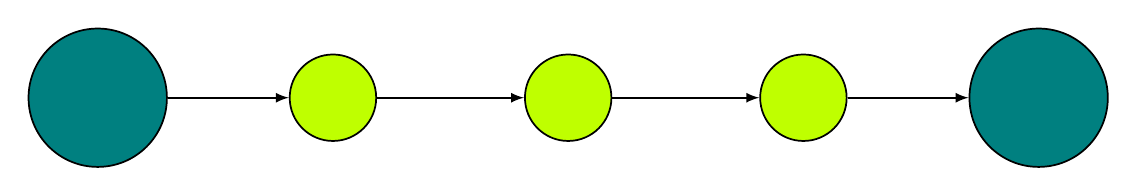
\begin{tikzpicture}
		[every node/.style={inner sep=0pt}]
		\node (1) [circle, minimum size=50.0pt, fill=teal, line width=0.625pt, draw=black] at (50.0pt, -130pt)  {};
		\node (2) [circle, minimum size=31.25pt, fill=lime, line width=0.625pt, draw=black] at (135pt, -130pt)  {};
		\node (3) [circle, minimum size=31.25pt, fill=lime, line width=0.625pt, draw=black] at (220pt, -130pt)  {};
		\node (4) [circle, minimum size=31.25pt, fill=lime, line width=0.625pt, draw=black] at (305pt, -130pt)  {};
		\node (5) [circle, minimum size=50.0pt, fill=teal, line width=0.625pt, draw=black] at (390pt, -130pt)  {};
		\draw [line width=0.625, ->, >=latex, color=black] (1) to  (2);
		\draw [line width=0.625, ->, >=latex, color=black] (2) to  (3);
		\draw [line width=0.625, ->, >=latex, color=black] (3) to  (4);
		\draw [line width=0.625, ->, >=latex, color=black] (4) to  (5);
		\end{tikzpicture}\\
		Let	us define the the properties of the incremental backup($B_I$) in a similar fashion:
		$$
		B_I
		\begin{cases}
			p_I: \text{the probability of failure}\\
			r_I: \text{the recovery trial cost}\\
			t_I: \text{the days between two consecutive incremental backups}\\
		\end{cases}
		$$
\newpage
		Let $T_F$ denote the difference in days between the disaster date and the successful full backup and $l$ denote the number of incremental backups we have to consider. We have two options for $l$ depending on whether the latest full backup was successful:
		$$
			l=
			\begin{cases}
				\left\lfloor \frac{T_F}{t_I}\right \rfloor \text{, if } T_F<t_F\\
				\left\lfloor \frac{t_F}{t_I}\right \rfloor -1 \text{, if } T_F>t_F\footnotemark\\
			\end{cases}
		$$
		\footnotetext{We can only try to recover incremental backups preceding the next full backup}
		Note that the last full backup being successful is equivalent to $T_F<t_F$.\par
		We are in the exact opposite situation with respect to the previous subsection. The process of recovering incremental backups continues until we conduct an unsuccessful attempt to recover the data, as this will mean none of the following backups can be used either. Note that we are reducing $W$ since in the initial position we are willing to redo the work up to the working full backup. That being said, we are ready to calculate the expected price:
		\begin{equation}
		\label{eq:2}
			f(T_F) = (1-p_I)^l.((T_F-t_I.l).w + r_I.l) + \displaystyle \sum_{i=0}^{l-1} (1-p_I)^{i}.p_I((T_F-t_I.i)w + r_I.(i+1))
		\end{equation}
		Now we know how much the price will decrease when we use incremental backups and can build the whole picture using equations \ref{eq:1} and \ref{eq:2}.
		\subsection{Overall expected price}
		For each summand in \ref{eq:1} we should add the effect of incremental backups, so we get new summands of the type:
		$$
		P(W + R),
		$$
		where $P$ is the probability of a certain combination of events occurring, $W$ is the cost of the data that has to be reworked and $R$ is the cost of the recovery process. Incremental backups lower the cost of the data that has to be reworked but make $R$ bigger. As mentioned before, there is only one case when the number of incremental backups we have to consider is different and it corresponds to the first full backup being successful. If the $i$-th full backup is successful\footnote{This corresponds to the $i-1$-th summand in the sum from equation \ref{eq:3}}:
		$$
		T_F=t_F\left(\left\{ \frac{T}{t_F} \right\} + i - 1\right)
		$$
		By combining equations \ref{eq:1} and \ref{eq:2} we get:
		\begin{equation}\label{eq:3}
			F(T) = p_F^{k}(W_T+k.r_F) + \displaystyle\sum_{i=0}^{k-1}(1-p_F).p_F^{i}\left(f(T_F) + (i+1).r_F\right)
		\end{equation}
		Using the described equations \ref{eq:1} and \ref{eq:3}, we can construct a graph of the expected price with and without incremental backups included.
		\begin{figure}[H]
			\begin{minipage}{1.0\textwidth}
				\centering
				\includegraphics[width=0.7\textwidth]{"Weekly_full"}
				\caption{Full only and Whole model}\label{Fig:FullWeekly}
			\end{minipage}
		\end{figure}
		\subsection{Monte Carlo simulation}
			A Monte Carlo simulation has been build with python to generate random recovery processes with the described conditions of backup structure. The price of the recovery has been graphed with respect to the disaster date:
			\begin{figure}[H]
				\begin{minipage}{1.0\textwidth}
					\centering
					\includegraphics[width=0.7\textwidth]{"Weekly_full_carlo"}
					\caption{Monte Carlo simulation}\label{Fig:MonteCarlo}
				\end{minipage}
			\end{figure}
		\blfootnote{In both Figure \ref{Fig:FullWeekly} and Figure \ref{Fig:MonteCarlo} the data showed is for a weekly full and daily incremental backups}
		The colors in Figure \ref{Fig:MonteCarlo} represent the type of the last backup, which was successful during the recovery, full, incremental or non-existing.
		\newpage
		A linear regression has been made of the data generated, which is to show that the effect of initial unsecured data fades with time, as the price of failure is calculated as the price to redo the whole work from the creation of the company.
		\subsection{Results}
			A model for backing up data has been built to calculate the expected price of backup recovery. Furthermore, the effect of incremental backups has been shown, as opposed to a strategy using only full backups. A Monte Carlo simulation has been built and analyzed to demonstrate the real process of recovery.
\section{Further development}
	The author considers several future development directions for the project, namely:
	\begin{itemize}
		\item considering non-constant work rate for the backup model
		\item expanding the ransomware model to describe more complex way of distributing the ransomware
		\item using the results and databases of related studies in order to back the project with real data\cite{paquet2019ransomware}
		\item considering a dynamic pricing model for the ransomware model
	\end{itemize}
\section{Acknowledgments}
I want to thank my mentor, Yavor Papazov, and Konstantin Delchev for the enormous help with the choice of the research subject and for providing me with all the necessary material to get familiar with the topic, as well as listening to my questions along the whole way. I extend my gratitude towards HSSIMI and SRS for the opportunity to develop this project and the irreplaceable atmosphere of dedication and concentration.
\bibliographystyle{unsrt}
\nocite{*}
\bibliography{Bibliography}
\end{document}